\subsection{Opsætning webapplikation udvikling}
Dette afsnit har til formål at beskrive hvordan et udviklingsmiljø sættes op på en givet maskine så videre udvikling af systemet kan finde sted. Afsnittet forklarer også hvilke tredjeparts teknologier der er anvendt og eventuelle afhængigheder der er brugt.

For at kunne opsætte et udviklings miljø til client applikationen, skal source koden først hente. Dette kan ske via git, skriv følgende kommando i terminalen.

\begin{lstlisting}[language=bash]
	$ git clone https://github.com/Opstrup/drone_frontend
\end{lstlisting}

\vspace{-1cm}

\subsubsection*{Mappestruktur}
Dette underafsnit vil forklare om den overordnede mappe struktur i webapplikation og give en overordnet forståelse af angular client udvikling. \\

På figur \ref{fig:mappestruktur_client} ses mappestrukturen for client applikationen. Da Angular frameworket er opbygget over MVC\footnote{MVC model i forbindelse med Angular: https://docs.angularjs.org/guide/databinding} modellen, er mappestrukturen opdelt så det afspejler denne model. I roden af projekt mappen findes to væsentlige filer, app.js og index.html. 
app.js er settings filen for projektet, i denne fil bliver alle afhængigheder af projektet hentet ind og initialiseret. States i applikationen og dertilhørende controllere bliver også registeret i app.js\footnote{Information omkring app.js indstillingerne: https://docs.angularjs.org/guide/introduction}.\\
index.html er som kendt fra webudvikling, den side der hentes først ved et request. Da Angular applikationer er opbygget med kun en side, fungerer det lidt anderledes. Når en side opbygget i Angular besøges, vil index siden blive hentet men der udover vil javascript- og css-filer også blive hentet. Via Angular frameworket bliver alle andre sider loaded ind i index siden, hvilket gøre applikationen hurtigt, idet filerne ikke skal indlæses igen.

\begin{figure}[H]
	\centering
	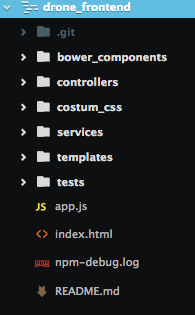
\includegraphics[width=0.3\textwidth]{Billeder/implementation/mappestruktur_client.png}
	\caption{Mappestruktur rod}
	\label{fig:mappestruktur_client}
\end{figure}

\newpage

\textbf{bower\_components}\\
I denne mappe findes alle tredje parts afhængigheder, i form af css og java script filer. Til håndtering af tredje parts teknologier er der benyttet bower\footnote{http://bower.io/}, som er et package manager program til webudvikling.

\textbf{controllers}\\
I denne mappe findes alle controller\footnote{https://docs.angularjs.org/guide/controller} i systemet, som fungerer på samme måde som kendt fra normal MVC.

\textbf{costum\_css}\\
Ud over bootstrap til håndtering af css'en, er der også blevet lavet små filer med css kode. Disse filer findes i denne mappe.

\textbf{services}\\
I denne mappe findes alle services\footnote{https://docs.angularjs.org/guide/services} i systemet. Disse services indeholder alt buisness logikken i systemet og derved fungere som models i MVC modellen.

\textbf{templates}\\
I denne mappe findes alle html filerne for systemet, disser filer danner sammen med controllerne de views som bliver præsenteret i browseren\footnote{https://docs.angularjs.org/guide/templates}.

\subsubsection*{Udviklingsmiljø}
Opsætning af et udviklingsmiljø til client applikationen er lige til. Source koden indeholder alt hvad der skal bruges for at kunne compile, der skal kun bruges en browser til at starte applikationen. Til videreudvikling af applikationen anbefales det at udvide med andre applikationer, for at gøre udviklingsarbejdet lettere.

\textbf{Text editor}\\
Som alt andet web udvikling foregår det hele i scripts som køres i browseren, derfor er der ingen specielle krav til et IDE. Nogle gode text editors til web udvikling er Sublime eller Atom\footnote{Yderligere beskrevet i afsnittet om Server Opsætning}.

\textbf{Lokal web server}\\
For at applikationen fungerer optimalt, er det at foretrække at der installeres en web server på udviklerens maskine. Der er ikke nogle specielle krav til hvilke slags server. En mulighed ville være at sætte en Apache server op. For at simplificere installationen og opsætningen kan XAMPP\footnote{https://www.apachefriends.org/index.html} benyttes. Et andet eksempel på en web server kunne være en node.js server\footnote{http://nodejs.org/}. 



\newpage

\textbf{Package management}\\
Som før nævnt er bower brugt til package management og det anbefales at der fortættes med dette da bower\footnote{http://bower.io/} selv downloader og installerer de påkrævede filer, så udvikleren ikke skal tænke yderligere over dette.  


\subsubsection*{Tredje parts teknologier}
Til udviklingen af web applikationen er der blevet brugt nogle tredje parts teknologier, som er beskrevet yderligere i dette underafsnit.

\textbf{bootstrap}\\
Det populære bootstrap\footnote{http://getbootstrap.com/} css framework er benyttet til at designe applikationen.

\textbf{ui-router}\\
Ui router\footnote{https://github.com/angular-ui/ui-router} er en applikation som er lavet til Angular frameworket som gør routing imellem diverse views meget simpel. 

\textbf{google-maps}\\
Google maps er blevet brugt til at vise kortet i webapplikationen. Via google maps bliver der hentet GPS-koordinater som dronen flyver efter. Standard Google maps API'et er ikke blevet benyttet, men et angular applikation\footnote{https://angular-ui.github.io/angular-google-maps/} er anvendt i stedet, da det fungerer bedre med det resterende kode.

\newpage